\documentclass[12pt]{article}
\usepackage[utf8]{inputenc}
\usepackage{hyperref}
\usepackage{graphicx}
\usepackage{amsmath}
\usepackage{listings}
\usepackage{xcolor}
\usepackage{geometry}

\geometry{
    a4paper,
    margin=1in
}

\title{BuildFair: A Decentralized Protocol for Secure Construction Agreements}
\author{BuildFair Team}
\date{\today}

\begin{document}

\maketitle

\begin{abstract}
BuildFair is a decentralized Ethereum protocol designed to facilitate secure and transparent construction agreements between buyers and sellers. By leveraging smart contracts, BuildFair automates payment processes and ensures fair transactions while maintaining immutable records on the blockchain. This whitepaper presents the protocol's architecture, implementation details, and security considerations.
\end{abstract}

\tableofcontents

\section{Introduction}
The construction industry often faces challenges related to payment security, work verification, and dispute resolution. Traditional contracts can lead to delayed payments, trust issues, and costly legal disputes. BuildFair addresses these challenges through blockchain technology and smart contracts, providing a trustless environment for construction agreements.

\section{Protocol Overview}
\subsection{Core Components}
\begin{itemize}
    \item Smart Contract System
    \item Project Management
    \item Payment Automation
    \item Work Verification
\end{itemize}

\subsection{Key Features}
\begin{itemize}
    \item Automated payment release upon work verification
    \item Secure fund escrow
    \item Transparent project tracking
    \item Immutable record keeping
\end{itemize}

\subsection{User Flows}
Figure 1 illustrates the interaction flows between different users in the BuildFair protocol.

\begin{figure}[h]
    \centering
    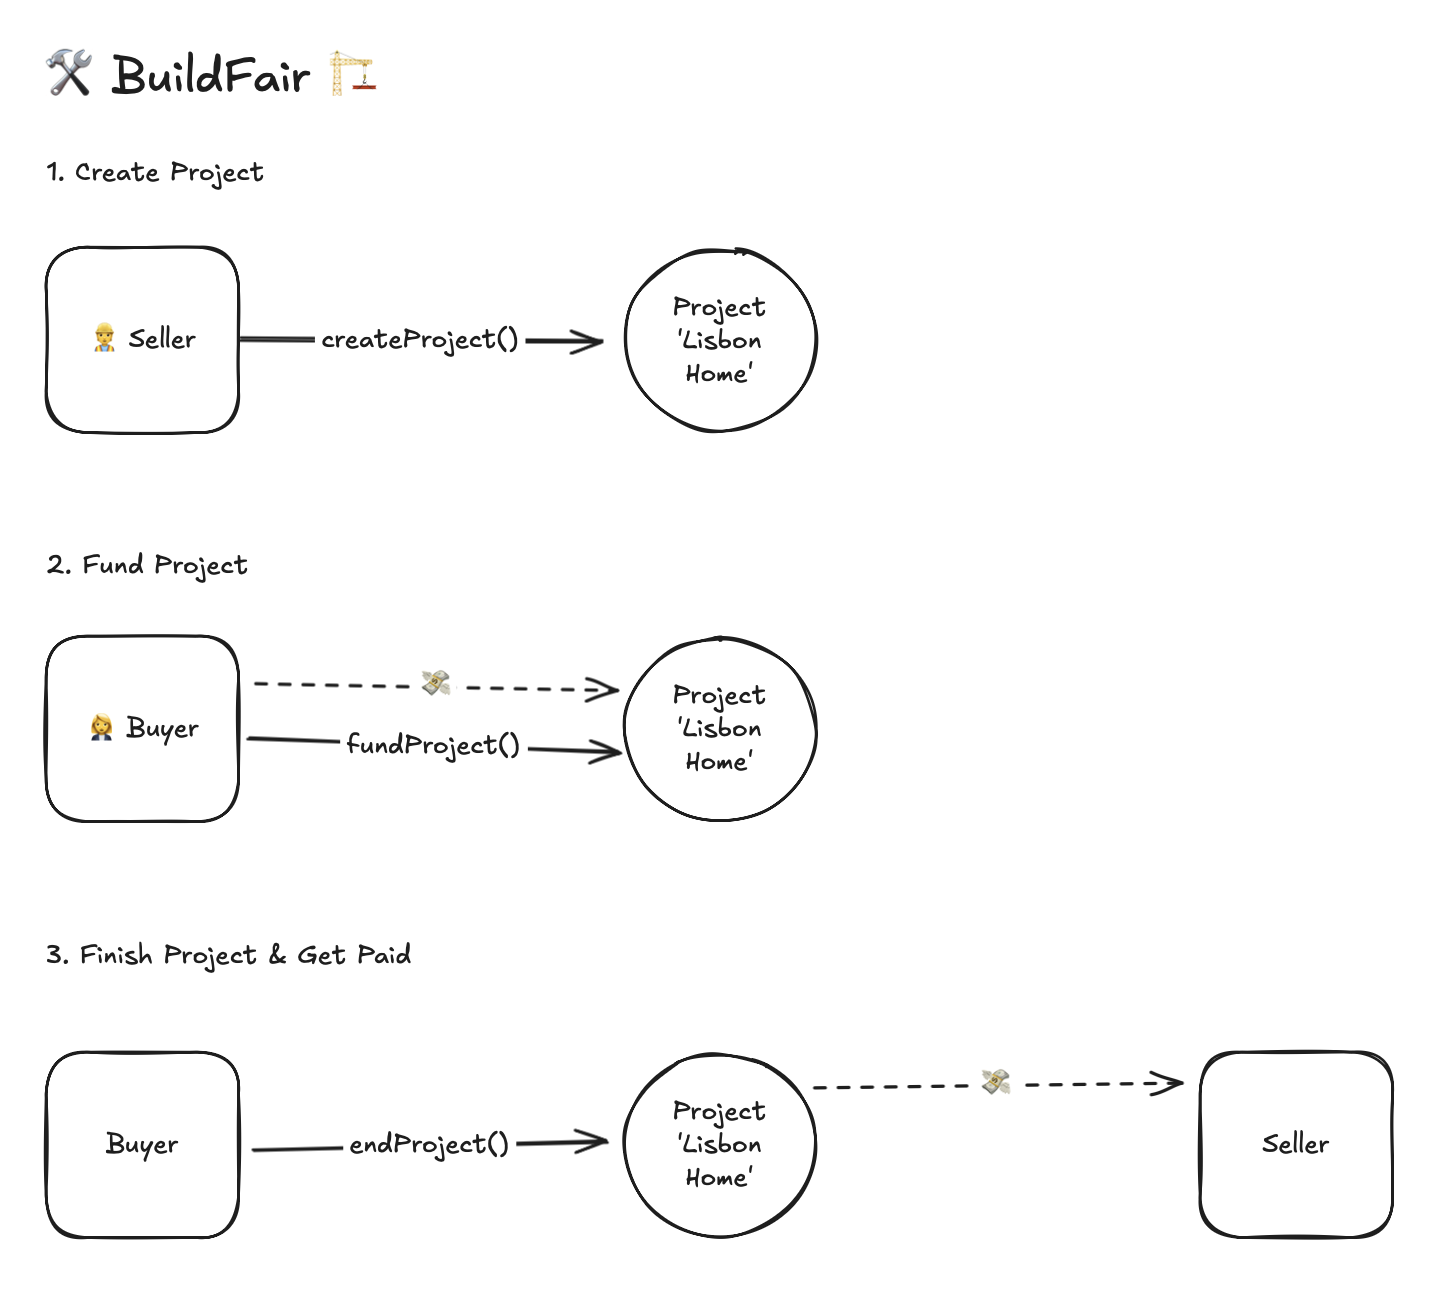
\includegraphics[width=\textwidth]{../buildfair-app/public/userflows.png}
    \caption{BuildFair User Interaction Flows}
    \label{fig:userflows}
\end{figure}

\section{Architecture}
\subsection{Smart Contract Design}
The BuildFair smart contract implements a state machine pattern with the following states:
\begin{itemize}
    \item Created: Initial project setup
    \item Funded: Buyer has deposited funds
    \item Ended: Project completion and fund distribution
\end{itemize}

\subsection{Role-Based Access Control}
The protocol defines three primary roles:
\begin{itemize}
    \item Buyer: Funds projects and approves work completion
    \item Seller: Executes construction tasks and submits completion evidence
    \item Future: Jury system for dispute resolution
\end{itemize}

\section{Technical Implementation}
\subsection{Smart Contract Functions}
\begin{lstlisting}[language=Solidity]
// Core Functions
function createProject(address seller, string details)
function fundProject(uint256 projectId)
function submitWork(uint256 projectId)
function approveWork(uint256 projectId)
function endProject(uint256 projectId)
\end{lstlisting}

\subsection{Project Lifecycle}
\begin{enumerate}
    \item Project Creation: Buyer initiates project with seller assignment
    \item Project Funding: Buyer deposits ETH into smart contract
    \item Work Execution: Seller performs construction work
    \item Work Verification: Buyer approves completed work
    \item Payment Distribution: Smart contract releases funds to seller
\end{enumerate}

\section{Security Considerations}
\subsection{Smart Contract Security}
\begin{itemize}
    \item Reentrancy protection
    \item Access control validation
    \item State transition verification
    \item Secure fund handling
\end{itemize}

\subsection{Future Security Enhancements}
\begin{itemize}
    \item Multi-signature requirements
    \item Time-locked operations
    \item Jury system implementation
    \item Dispute resolution mechanism
\end{itemize}

\section{Future Development}
\subsection{Planned Features}
\begin{itemize}
    \item Milestone-based payments
    \item Jury system for dispute resolution
    \item Enhanced evidence submission system
    \item Multi-party project support
\end{itemize}

\subsection{Protocol Upgrades}
\begin{itemize}
    \item Governance implementation
    \item Protocol fee structure
    \item Cross-chain compatibility
    \item Layer 2 scaling solutions
\end{itemize}

\section{Economic Model}
\subsection{Token Economics}
Future iterations may include:
\begin{itemize}
    \item Protocol governance token
    \item Staking mechanisms
    \item Jury incentivization
    \item Fee distribution model
\end{itemize}

\section{Conclusion}
BuildFair represents a significant step forward in modernizing construction agreements through blockchain technology. By providing a secure, transparent, and automated platform, the protocol addresses key challenges in the construction industry while laying the groundwork for future enhancements and expanded functionality.

\section{References}
\begin{enumerate}
    \item Ethereum Yellow Paper
    \item Smart Contract Best Practices
    \item Construction Industry Payment Standards
    \item Blockchain-based Payment Systems
\end{enumerate}

\end{document}